\documentclass[autodetect-engine,dvipdfmx-if-dvi,ja=standard,a4paper,layout=v2]{bxjsreport}
\usepackage{ifxetex,ifluatex}
\usepackage{unicode-math}
\setmainfont[Ligatures=TeX]{TeXGyreTermes}
\setsansfont[Ligatures=TeX]{TeXGyreHeros}
\setmonofont{Inconsolatazi4}
\usepackage{graphicx, amsmath, cite, ascmac, amsfonts}

\makeatletter
\newcommand{\tref}[1]{Table.~\ref{#1}}
\newcommand{\eref}[1]{Eq.~(\ref{#1})}
\newcommand{\fref}[1]{Fig.~\ref{#1}}
\renewcommand{\theequation}{
  \thesection.\arabic{equation}}
\@addtoreset{equation}{chapter}
\def\theequation{\thechapter.\arabic{equation}}
\def\cite#1{\textsubscript{#1}}
%\def\section{\newpage\@startsection {section}{2}{\z@}{3truemm}{3truemm}{\Large\bf}}
\makeatother


\author{前田大輝}
\title{周期ポテンシャルにおける波束の時間発展}
\begin{document}
    \maketitle
    \begin{abstract}
        周期ポテンシャルは一定の周期構造を持つ分子の並びをモデル化したものであり、
        中でも最も簡単なKronig-Pennyモデルでは定常状態のエネルギーバンド構造を説明することができる。
        一方で時間に依存した現象では、波束が時間の2乗よりも早く緩和することが知られており、
        Heyperdiffusionと呼ばれている。
        このような、周期ポテンシャル中の粒子が真空中とは違った振る舞いをすることに関する知見は、
        固体物理やナノリソグラフィなどの分野に応用できる場合がある。
        そこで本研究は、特定の(半)周期ポテンシャルにおける波束が
        どのように緩和していくのかを解析することを目的として、
        主にコンピュータにおける数値計算的な手法を用いている。
        その結果Kronig-Penny型の周期ポテンシャルに入射する波束は、
        ステップ型のポテンシャルに入射した場合と比べて、
        反射波に遅れが生じることを発見した。
    \end{abstract}
    \tableofcontents
    \chapter{研究の目的}
    \begin{chapterabstract}
        物質中の電子は真空中と比べ、特異な振る舞いをすることが知られている。
        その代表例が結晶内におけるエネルギーバンド構造であり、結晶中の電子は連続したエネルギースペクトルを持つことができない。
        バンドギャップにあたるエネルギー状態をとる電子は結晶境界で全反射するか、ギャップ分のエネルギーを光子として放出し、
        バンドに適合したエネルギーを持って物質中に侵入する。\par
        この物理現象について、定常状態での解析はなされているが、時間依存の詳細についてはまだ未解明である。
        近年は光格子時計により時間分解能が飛躍的に向上しているため、現在の「一瞬にしてバンド構造が作られる」という近似が
        成立しなくなる可能性がある。そこで、どの程度の時間分解能ならばその近似が成立するかの目安を求めること重要性が増している。\par
    \end{chapterabstract}
    \section{波束の時間発展}
    波束とは局在化した波動のことで、量子波束は古典的な質点に対応する。
    例えば、十分に細い電子パルスは古典的に点粒子とみなすことができる。
    分解能$d$と位置不確定性$\delta x$との関係\eref{acc}が、波束と質点を対応させる古典近似の成立条件となる。
    \begin{itembox}[l]{古典近似成立条件}
      \begin{align}
        \frac{\delta x}{d} \ll 1 \label{acc}
      \end{align}
    \end{itembox}
    しかし、古典近似は時間とともに成立しなくなる。
    これは、自由量子波束が本質的に時間依存した現象であることに由来している。
    つまり、静止した自由粒子は古典的には定常的で時間依存しないが、
    一般にSchrödinger方程式における静止\footnote{
      重心が移動しない
    }自由波束は時間とともに緩和するため、
    $\delta x$は時間とともに増加し、\eref{acc}が成立しなくなる。\par
    $\delta x$の目安として標準偏差$\sigma(t)$を使うと、Gauss型波束の場合、$\sigma(t)$は次の\eref{SD}で表せる。
    \begin{align}
      \sigma(t) = \sigma_0 + \alpha t \label{SD}
    \end{align}
    $\sigma_0$は初期状態の標準偏差で、$\alpha$は質量と$\sigma_0$に依存する正の定数を意味している。
    \eref{SD}よって、一様ポテンシャル中あるいは真空状態での古典近似が成立する条件
    \eref{acc}の陽に時間依存した形を得ることができる。\par
    \begin{align}
      \frac{\sigma_0 + \alpha t}{d} \ll 1
    \end{align}
    $t=0$のときには\eref{acc}が成立しているとして時間の一次についてのみとると、
    \eref{acc}が成立する限界時間$\delta t_{lim}$はおおよそ\ref{acc2}で表される。
    \begin{align}
      \frac{\alpha}{d} \delta t_{lim} \sim 1 \nonumber\\
      \delta t_{lim} \sim \frac{d}{\alpha} \label{acc2}
    \end{align}
    しかし、\eref{SD}は前提として力が加わっていない状態を仮定している。
    よって、この式から直ちに一般の場合について古典近似が成立する時間の目安を見いだすことはできない。
    そこで、真空以外の場合、中でも特に物質中のポテンシャルについて、この目安を見出すことには一定の意味がある。
    \begin{itembox}[l]{波束についてのまとめ}
      \begin{itemize}
        \item 波束は古典近似で質点に対応する
        \item 波束は時間発展とともに緩和する
        \item 物質中での緩和速度についてはよくわかっていない
      \end{itemize}
    \end{itembox}
    \section{Kronig-Pennyモデル}
    結晶中でエネルギー固有状態にある電子は取り得るエネルギーに飛躍が現れる。
    この構造のことをエネルギーバンド構造という。
    エネルギーバンド構造は結晶の並進対称性と関連がある。\par
    Blochは、結晶原子が周期的に並んでいる構造を、ポテンシャルが周期的に並んでいる構造と対応させて、
    周期ポテンシャル中の波動関数が従う一般的な形式\eref{BlochTheorem}を求めた。
    \begin{itembox}[l]{Blochの定理}
      \begin{align}
        \phi(x) = u(x) \mathrm{e}^{-k x} \label{BlochTheorem}
      \end{align}
    \end{itembox}
    $k$は逆格子ベクトルと呼ばれる結晶の周期に依存する定数、$u(x)$は結晶と同じ周期をもつ関数で結晶構造に依存する。
    周期ポテンシャル中の波動関数が\eref{BlochTheorem}に従うという定理をBlochの定理と呼ぶ。\par
    この定理を使って、KronigとPennyはポテンシャルが\eref{defKP}のように表される場合に、
    エネルギーバンド構造が形成されることを説明した。
    \begin{itembox}[l]{Kronig-Pennyポテンシャル}
    \begin{align}
        V_{KP}(x) =
        \begin{cases}
          V_0  & (0 \leq x \leq a)\\
          0    & (a \leq x \leq d)\\
          V_{KP}(x - d) & (otherwise)
        \end{cases}\label{defKP}
      \end{align}
    \end{itembox}
    \eref{defKP}は箱型ポテンシャルが周期的に並んだ構造を表している。
    これは周期ポテンシャルの中でも最も単純な具体例の一つで、Kronig-Pennyポテンシャルと呼ばれる。
    結晶をKronig-Pennyポテンシャルで表現するというモデルは
    簡単な構造ながらエネルギーバンド構造を説明することができる点で有効であり、Kronig-Pennyモデルと呼ばれる。\par
    また、定常状態についての構造は古くから知られているKronig-Pennyポテンシャルだが、
    非定常状態はBlochの定理が成立しないため、波動関数が\eref{BlochTheorem}で表されることはない。
    これに関しては、Hunagel、Zenjunによって確率供給源からの量子拡散についての研究\footnote{
      Zhanのポテンシャルは$x=0$付近だけ井戸の間隔が広くなっている
    }が行われている。
    この結果、波束の標準偏差が時間に比例するよりも早く大きくなる現象が見出され、Heyperdiffusionが起こることを示した。\par
    このように、物質中の波束や真空中の波束についてはある程度の知見が得られているが、
    真空中から物質中に入射する波束については未だ知見が得られていない。
    この場合、暗黙に真空中では波束とみなし、結晶中でエネルギーバンド状態であるとみなす近似\footnote{
    古典的には、電子が物質に侵入すると物質全体の電位がほとんど一瞬で上昇することと対応している。
    }が行われる。
    しかし、波束は非定常状態であり、エネルギーバンド状態は定常状態であるため、
    厳密には2つの状態間を一瞬で移り変わるわけではない。
    時間分解能が高まった現代では、結晶に入射した波束が拡散しながらエネルギーバンドを作る過程が観測にかかる可能性がある。
    よって、エネルギーバンド構造が作られる時間の目安を与えることには一定の意味がある。\par
    そこで、エネルギーバンドの構成時間を調べるために、最も簡単な周期ポテンシャルであるKronig-Pennyモデルを用いて解析を行う。
    またKronig-Pennyモデル自体がナノリソグラフィーの素子や半導体超格子に対する良い近似として成立しているため、
    それらの性質を知る上で、この研究は実際的な研究となる。
    \begin{itembox}[l]{Kronig-Pennyモデルについてのまとめ}
      \begin{itemize}
        \item 物質中の電子は定常状態でエネルギーバンド構造を作る
        \item Kronig-Pennyモデルはエネルギーバンド構造を説明できる
        \item 真空からKronig-Pennyポテンシャルに入射する波束の緩和についてはよくわかっていない
      \end{itemize}
    \end{itembox}
    \chapter{数値計算}
    \begin{chapterabstract}
        Kronig-Pennyポテンシャル中のGauss型波束の時間発展を解析的に得ることは非常に困難を伴う。
        そのため、近似的な方法を用いる必要がある。
        しかし、Schrődinger方程式は二階の偏微分方程式であり、計算機で解くには少し工夫がいる。
        そこで、複数の方法を検討し、妥当な方法を提案する。
    \end{chapterabstract}
    \section{Euler法}
    この節は主に学部生に対して、常微分方程式を数値的に解くことの雰囲気を知ってもらうことを目的としている。
    形式的な話が多いが、それはどんな方程式にも対応できるように問題を抽象化しているからで、
    ”どんな難しい方程式も解くことができる”という数値計算の力強さの源になっている。
    枝葉の些事は気にせず、大雑把に何をやっているのかを知ってほしい。\par
    一階の常微分方程式は一般的に\eref{diffEQ1}、\eref{diffEQ2}の形で表すことができる。
    \begin{align}
      \frac{dy}{dt} = f(y,t)\label{diffEQ1}\\
      y(t_0) = y_0\label{diffEQ2}
    \end{align}
    ここで$y_0$は初期条件として与えられる既知の値とする。
    \eref{diffEQ1}の右辺を積分し、積分定数として\eref{diffEQ2}を使えば、この方程式の解が得られる。
    しかし、計算機で数値的に解く際にこの方法は使うことができない。
    なぜなら、計算機は有限回の加減乗除\footnote{
      厳密に言うと二進数のビットシフト、AND,OR,NOT演算の組み合わせ
    }しか扱うことができないからである。
    形式的な微積分操作をプログラムしてやることで対応可能な場合もあるが、その場合は人間が手で解くのとあまり変わりがない。
    今考えたいのは、解析的に解くことができない場合\footnote{
      例えば$f(y,t)=y^t$のとき
    }である。\par
    解析的手段が使えない場合、微分方程式の解析解を得る手段がないため、問題の設定を変更する。
    解析解を得ることは諦め、解の条件を少し緩めて、任意の精度で真の値に近い値を得ることができればよいことにする。
    そこで、無限回の計算を有限回で打ち切るような近似を行い、計算機でも可能にする。\par
    近似方法は多岐にわたるが、数値計算の数ある方法の中でも、この節の目的達成に最も適した方法としてEuler法を取り上げる。
    あまり実用的な方法ではないが、数値計算特有の難しさや、力強さを掴んでもらうためには十分だと考えている。
    なぜなら最も基礎的な\footnote{
      ”基礎的であること”と”簡単なこと”は同じではない。
      基礎を生み出すことは、応用することとは違った難しさがある。
    }計算方法だからである。
    この方法を発展させた方法はRunge-Kutta法と呼ばれ、最もメジャーな数値計算法のクラスを作っている。\par
    Euler法は、$y(t)$を$t=0$の周りでTaylor展開\footnote{
      Taylor展開できる関数には$C^\infty$級(定義域のすべての点で無限回微分可能)という制約が付いているが、
      物理で使う関数はだいたい微分可能なのであまり心配はいらない。
    }することで得られる。
    \begin{align}
      y(t) = y(t_0) + \left.\frac{dy}{dt}\right|_{t=t_0}\!(t-t_0) 
      + \frac{1}{2}\left.\frac{d^2y}{dt^2}\right|_{t=t_0}\!(t-t_0)^2 + \dots\label{Ytaylor1}
    \end{align}
    $t$についての一次の項は\eref{diffEQ1}の$f(y,t)$を使い、ゼロ次の項は\eref{diffEQ2}を使って表すことができる。
    そして、二次以降の項は$t=t_0$の近傍では無視できるとすると、$h \ll 1$において\eref{EulerMethod1}が成立する。
    \begin{align}
      y(t_0 + h) \simeq y_0 + f(y_0,0)h = y_1 \label{EulerMethod1} 
    \end{align}
    これによって、既知の値$y_0$から、未知の値$y(t_0 + h)=y_1$を得ることができた。
    次に$t=t_0 + h = t_1$の周りでTaylor展開を行うと、\eref{Ytaylor1}とよく似た\eref{Ytaylor2}を得ることができる。
    \begin{align}
      y(t) = y(t_1) + \left.\frac{dy}{dt}\right|_{t=t_1}\!(t-t_1) 
      + \frac{1}{2}\left.\frac{d^2y}{dt^2}\right|_{t=t_1}\!(t-t_1)^2 + \dots\label{Ytaylor2}
    \end{align}
    そして、\eref{EulerMethod1}と同様にすると\eref{EulerMethod2}が得られる。
    \begin{align}
      y(t_1 + h) \simeq y_1 + f(y_1,t_1)h = y_2\label{EulerMethod2} 
    \end{align}
    これらの操作を次々に繰り返すことで、$t=t_n$における$y(t)$の値を求めることができる。
    ここまでの議論で十分だが、一応常微分方程式\eref{diffEQ1}、\eref{diffEQ2}における
    Euler法の定義を書いておくと次のようになる。
    \begin{itembox}[l]{Euler法}
      \begin{align}
        y_{n+1} = y_n + f(y_n,t_n)h\label{EulerMethod}
      \end{align}
    \end{itembox}
    \eref{EulerMethod}では、$f(y_n,t_n)$の計算を除くと1回の掛け算と1回の足し算しか使っていないため、
    有限回の加減乗除しかできない計算機でも計算することができる。
    この方法を使えば、どんな方程式でも理論上、計算機で解くことができる。\par
    しかし、$h$の値によってはTaylor展開の高次の項を無視することができないため、計算誤差が発生する。
    1ステップでの誤差の大きさは、Euler法では概ね$h$に比例する。
    そのため、有効数字を1桁上げるためには、ステップ幅$h$を10分の1にしなければならず、10倍のステップ数が必要になってしまう。
    ”理論上は”どんな方程式も任意の精度で解くことができる\footnote{
      実際は丸め誤差の影響で、任意の精度で求めることはできない。
    }が、それは自分が生きている間とは限らない。
    \begin{itembox}[l]{Euler法のまとめ}
      \begin{itemize}
          \item 数値計算は近似的に解を求める
          \item どんな方程式も解くことができる
          \item 生きている間に計算が終わるとは限らない
      \end{itemize}
    \end{itembox}
    \section{数値計算法決定における指標}
    数値計算の方法はバラエティが豊かだが、基本的に安定性、計算量の2つが重要な指標となる。
    これらは数値計算特有の困難を数値化したもので、安定性は計算誤差、計算量は資源の消費量を表す指標となる。\par
    計算誤差の具体例として、丸め誤差と打ち切り誤差を挙げる\footnote{
      他に数値計算に影響を与える誤差として連続量を離散量で表す際に発生する離散化誤差がある。
    }。\par
    計算機は基本的に実数を直接扱うことができないため、一定の精度で近似をして計算する。
    このような計算機の精度による誤差を丸め誤差という。
    具体的には、割り算、平方根が有限桁で表せない場合に有限桁の”小数”で近似を行うため、丸め誤差が発生する。
    ここで言う”小数”は二進数における小数であって、十進数における小数ではない。
    例えば、十進数における$0.1$を入力した場合、計算機の内部で丸め誤差が発生する。
    なぜなら、0.1は二進数においては\eref{DtoD}で表せるように無限小数となるためである。
    \begin{align}
      0.1 \qquad \mathrm{(on \: decimal})
      &= 2^{-4} + 2^{-5} + 2^{-8} + 2^{-9} + 2^{-12} + \quad \dots \qquad\mathrm{(on \: decimal)} \nonumber\\
      &=0.0\: 0011 \: 0011 \: 0011 \: 0011 \: \dots \qquad \mathrm{(on \: binary)} \nonumber\\
      &=0.0\: \dot{0} \dot{0} \dot{1} \dot{1} \qquad \mathrm{(on \: binary)}\label{DtoD}
    \end{align}
    よって、計算機で数値計算を行う際には、丸め誤差は必然的に発生する。\par
    また、有限時間で計算を終えるためには、無限数列を有限の項で打ち切らなくてはならない。
    例えば、\eref{Napier}を使って、Napier数$\mathrm{e}$を計算することができる。
    \begin{align}
      \mathrm{e} = \sum_{n}^{\infty} \frac{1}{n!} \label{Napier}
    \end{align}
    しかし、計算機では$n$について無限に足し合わせることはできない。
    よって、有限項(例えば1000項)で打ち切る近似を行い、\eref{NapierLess}を計算する。
    \begin{align}
      \mathrm{e} &= \sum_{n}^{\infty} \frac{1}{n!} \nonumber\\
      &\simeq \sum_{n}^{1000} \frac{1}{n!} \label{NapierLess}
    \end{align}
    この計算の一行目から二行目に移るところでは高次の項の寄与\footnote{
    もちろん、1000項ではなく5000項の方が高い精度を期待できるが、計算に時間がかかるため、
    いずれにしても\eref{Napier}を直接計算する方法では無限の精度の計算を有限の時間で行うことはできない。
    }が打ち切られているため、真の値よりも小さくなってしまう。
    このように打ち切り誤差は必然的に発生する。\par
    計算誤差は避けようがないが、制御することはできる。
    常微分方程式の数値解法では、積分範囲を有限区間に区切って積分を行うが、
    このステップ幅を小さくすれば精度は高くなる\footnote{
      ステップ数が増えると、丸め誤差の発生が多くなるため、いくらでも精度が高くなるわけではない。
      よって、計算量を無視しても、やはりアルゴリズムによって適度なステップ幅が存在する。
    }。
    そこで、どの程度のステップ幅ならば許容できるのかが重要になってくる。
    これを議論するときに必要なものが安定性の概念である。\par
    常微分方程式\eref{testEQ1}\eref{testEQ2}を一定の刻み$h$で数値積分するとき、解が必ず真の値に収束する
    \footnote{丸め誤差を無視する}ような$\lambda h$が存在する場合がある。
    この$\lambda h$が取り得る領域を絶対安定領域という。
    \begin{align}
      \frac{df}{dx}= \lambda f(x)\label{testEQ1}\\
      f(0) = y_0\label{testEQ2}
    \end{align}
    安定性は、この絶対安定領域の広さによって議論することができる。
    絶対安定領域の広さについて経験的に知られていることとして、陰的公式\footnote{
      $t=t_n$における$f(t_n)$を計算する際に$f(t_n)$の値を必要とする。
      つまり、すべての$n$についての連立方程式を解くことで解を得る方法。
    }のほうが広く、陽的公式\footnote{
      陰的公式とは逆に、$t=t_n$における$f(t_n)$を計算する際に$f(t_n)$の値を必要としない。
      このおかげで、逐次代入を行うだけで解が得られる。Euler法はこちら側の方法。
    }のほうが狭い。
    絶対安定領域はアルゴリズム固有のもので、アルゴリズムの良し悪しを決める際の指標となる。
    また、どのような$\lambda h<0$をとっても解が真の値に収束することをA安定というが、
    A安定だからといって実用的な時間でよい解が得られるとは限らない。\footnote{
      例えばEuler法を時間について逆向きにした陰的Euler法はA安定だが、
      局所的な誤差はEuler法とほぼ同程度で、ろくな精度が得られない。\\
      絶対安定領域とは、長時間計算を行っても数値解が真の値から大きくずれることはないステップ幅の領域を意味している。
    }
    収束性や計算の容易さは別の概念で測る必要がある。\par
    ただし、絶対安定領域が狭いアルゴリズムは、高い精度で計算しなければ計算が安定しないため、
    自分のほしい精度と絶対安定領域との2つを管理しなければならない分、難易度は上がる。\par
    計算量には、空間的計算資源(メモリ消費量)と時間的計算資源(計算時間)の消費量という2つの意味を持つが、
    2つの量は大まかに比例する傾向にある\footnote{
      もちろん、メモリを大量に消費して計算時間を短くしたり、その逆をしたりすることもあるが、
      大規模な計算に大量の資源が必要なことに変わりはない。
    }ため、今回は特に計算時間のことを指して「計算量」という言葉を用いる。
    計算量はプログラムに入力される情報の量$n$に依存するが、必ずしも入力情報量が二倍になると、計算量$\tau$も二倍になるとは限らない。
    入力情報に偏りがある場合\footnote{
      極端な例では、入力がすべて”1”だとわかっている場合、入力情報を愚直に\\
      \texttt{input(1,\: 1,\: 1,\: 1,\: 1,\: 1,\: 1,\: 1,\: 1,\: 1)}\\
      と記憶するのではなく、\\
      \texttt{input(1).times(10)}\\
      と回数だけ記憶すれば、1000個の入力だろうが、10000個の入力だろうが、
      定数のオーダーに圧縮することができる。
    }は$\tau$を小さく抑えることができる。
    また、入力情報のすべての組み合わせについて計算するようなアルゴリズムの場合は、$n$が増えると爆発的に$\tau$が増える。
    そこで、$\tau$の目安としてLandauの記号\eref{Landau}を用いることが多い。
    \begin{itembox}[l]{Landauの記号}
      \begin{align}
        \tau(n) = O(f(n)) \label{Landau}
      \end{align}
    \end{itembox}
    この記号は\eref{LandauDef}が収束することと等価である。
    \begin{align}
      \lim_{n\to\infty}\left|\frac{\tau(n)}{f(n)}\right| \label{LandauDef}
    \end{align}
    例えば、この記号を使うと$\mathrm{cos}(x)$はTaylor展開を使って次のように書ける。
    \begin{align}
      \mathrm{cos}(x) = 1 + O(x^{2})
    \end{align}
    この記号を使うと具体的な関数はわからなくても、大まかな傾向を見取ることができる。
    計算量もアルゴリズム固有の値をとり、アルゴリズムの良し悪しを決める指標となる。\par
    基本的に計算量が少なく絶対安定領域が広いアルゴリズムが求められるが、両方が優れている方法は存在しないため、
    適度なものを選ぶしかない。
    \begin{itembox}[l]{数値計算の指標}
      \begin{itemize}
        \item 絶対安定領域:計算が収束する誤差の範囲
        \item 計算量:計算にかかる時間
        \item 絶対安定領域と計算量はトレードオフ
      \end{itemize}
    \end{itembox}
\newpage
    \section{Fourie変換法}
    数値的にSchrődinger方程式を解く方法には大きくFFT法と有限要素法が存在する。
    Fourie変換法はエネルギー固有状態$\phi_n(x)$の重ね合わせによって系の初期状態$\psi_0(x) = \psi(x, t)|_{t=0}$を構成する。\par
    $\phi_n(x)$による$\psi_0(x)$の内積\footnote{
      単に片方の複素共役をとって積分しているだけなのでビビらないで欲しい。
    }が収束すると仮定する\footnote{
      $L^2$とよばれる関数空間の元だという仮定を置いている。\\
      物理的に言うと、\eref{combolution}は\\
      ”$\psi_0$の状態にある粒子の状態を観測したとき、その状態が$\phi_n$である確率が$C_n$である”\\
      ということを意味している。
      観測をすることができるということを仮定しているだけなので、
      あまり心配しないでもいい。
    }と、\eref{combolution}によってFourie係数が得られる。
    \begin{align}
      \int_{c}\phi^*_n(x)\psi_0(x)\quad dx = A_n\label{combolution}
    \end{align}
    よってFourie逆変換によって$\psi_0$と$\phi_n$の関係が\eref{FFT1}得られる。
    \begin{align}
      \Bigl.\psi(x, t)\Bigr|_{t=0} = \sum_{n}^{\infty} A_{n} \phi_n(x)\label{FFT1}
    \end{align}
    時間発展を計算したければ、角振動数$\omega_n$をエネルギー$\varepsilon_n$に応じて
    $\varepsilon_n / \hbar$で与えれば良い。
    \begin{itembox}[l]{Fourie変換法}
    \begin{align}
      \psi(x,t)=\sum_{n}^{N}\:A_n\ \phi_n(x) \:\mathrm{e}^{\frac{\varepsilon_n}{i\hbar} t}\label{FFT}
    \end{align}
    \end{itembox}
    この方法では、$\phi_n$がわかってしまえば、$O(1)$で計算することができる。\par
    計算誤差は主に\eref{FFT}の和を有限項で打ち切ることによって発生する。
    この相対誤差は低周波領域で顕著なため、$t$が大きな時間発展を計算する際は誤差が大きくなるが、
    小さい場合にはかなり効率がいい。
    また、あらゆる時刻の時間発展を計算する場合でも定数時間で計算が終了するという点でも非常に性質が良い。\par
    ただし、Kronig-Pennyポテンシャルにおける定常状態のSchrődinger方程式は、Diracの櫛と呼ばれる極限を除いて、
    解析的に解を得ることに計算精度の面で困難がある。
    そこで、本研究では解析的に定常状態を得ることは避け、数値的に定常状態を得るだけに留めることにする。
    \begin{itembox}[l]{Fourie変換法についてのまとめ}
      \begin{itemize}
        \item 定常状態を重ねあわせて計算する
        \item $O(1)$で計算できる(すごい!)
        \item 定常状態をどうやって求めるかはわからない
        \item Kronig-Pennyモデルでの定常状態は実質的に求められない
      \end{itemize}
    \end{itembox}
    \section{有限要素法}
    もうひとつの数値解法である有限要素法は積分する範囲を有限の区間に分割し、
    分割した区間内での解は適当な可積分関数\footnote{
      基本的に多項式だと考えて良い
    }で表せると近似することで、数値解を得る方法である。\par
    この方法のバリエーションとしてRunge-Kutta法と線形多段法が存在する。
    \subsection{Runge-Kutta法}
    Runge-Kutta法は積分したい点の近傍で線形近似を行い\footnote{
      つまり一階微分は定数だと近似する。
    }、補正を繰り返しながら何度も計算し直す方法で、Euler法はこのクラスに属する。\par
    例えば、二次関数$y(t) = \alpha t^2+\beta t+\gamma$を$t_a$と$t_b$の地点で正しくなるよう線形近似する場合を考える。
    傾きを直接計算すると\eref{example1}のようになるが、これは$t=(t_b+t_a)/2$、つまり二点の中間点での傾き\eref{example2}に
    等しい。
    \begin{align}
      \frac{y(t_b)-y(t_a)}{t_b-t_a}&=\dfrac{(\alpha t_b^2+\beta t_b+\gamma)-(\alpha t^2_a+\beta t_a+\gamma)}{t_b-t_a} \nonumber \\
      &=\alpha (t_b+t_a) + \beta\label{example1}\\
      &=2\alpha\left(\frac{t_a + t_b}{2}\right) + \beta \label{example2}
    \end{align}
    よって、\eref{diffEQ1}での$y(t)$について二次の項まで正しい式を作るためには
    区間の端点ではなく、中間地点での傾きを採用すれば良い。
    区間の中間地点を求めるときは、Euler法を用いる。
    これが2階2次の陽的Runge-Kutta法\footnote{
      中間地点を求めるためのEuler法(1回め)と、
      中間地点の傾きを使った線形近似(2回め)とで、合計2回の線形近似を行う方法なので”2階”(誤字ではない)のRunge-Kutta法といい、
      同時に2次のTaylor展開までと等しいので2次のRunge-Kutta法という。
      今回は階数と次数が一致したが、一般には階数のほうが大きくなる。\\
      また、あまり聞かないが、Euler法は1階1次のRunge-Kutta法ということができる。
    }の一種である。\par
    \begin{itembox}[l]{2階2次のRunge-Kutta法}
      \begin{align}
        y_{n+1}&=y_n + k_2h\\
        k_2&=f(y_n+k_1h/2,\:t_n+h/2)\\
        k_1&=f(y_n+h,\:t_n+_h)
      \end{align}
    \end{itembox}
    Runge-Kuttaの陰的方法には任意の次数でA安定の方法が存在するが、実用することは難しい。
    陰的方法を解くには一般に非線形連立方程式を解かなくてはならない。
    これを解くことは一階常微分方程式を解くことと同等か、それ以上に難しいためである。\par
    一方、Runge-Kuttaの陽的方法は逐次代入によって解くことができるため非常に計算が容易\footnote{
      トライアンドエラーの数をこなせるという意味で非常に重要な性質
    }である。
    また、以前のステップの情報を使わないため、ステップ幅を自由に変えることができるのも利点のひとつである。
    しかし、階数をあげても次数はあまり上がらない。また、絶対安定領域が非常に狭いか、存在しない。\par
    \subsection{線形多段法}
    一方、線形多段法は積分したい関数をRagrange補間などによってべき級数に近似する方法で、
    予測子修正子Adams法やAdams-Bashforth法などが知られている。\par
    Euler法は過去の値$y_n$ひとつから未来の値$y_{n+1}$を予測するが、もうひとつ過去の値$y_{n-1}$覚えておけば
    改良できるのではないかという発想で線形多段法は作られている。
    $y_n,y_{n-1}$が既知だとすると、$y_n$の周りで$f(y,t)$は\eref{linerIP}のように線形近似できる。
    \begin{align}
      f(y, t)
      &\simeq \frac{t-t_{n-1}}{t_n-t_{n-1}}f(y_n, t_n)+ \frac{t-t_{n}}{t_{n-1}-t_n}f(y_{n-1},t_{n-1}) \nonumber\\
      &=\frac{f(y_n,t_n)}{h}(t-t_{n-1}) - \frac{f(y_{n-1}, t_{n-1})}{h}(t-t_{n})\label{linerIP}
    \end{align}
    $t_n-t_{n-1}$はステップ幅に等しいので$h$と置いた。\par
    \eref{linerIP}のように多項式補間する方法をRagrange補間
    \footnote{
    複雑に見えるが、分解すると非常に簡単な原理で作られている。\par
    \begin{itemize}
          \item \underline{任意の$N$点$(y_0, t_0), (y_1, t_1),\dots ,(y_i,t_i),\dots ,(y_N,t_N)$を通る多項式}
            \begin{itemize}
               \item[$\hookrightarrow$] \underline{$t_i$以外の$t=t_1,t_2,\dots,t_N$では0を通り、$(y_i,t_i)$を通る多項式}を$N$個重ねあわせた多項式
                 \begin{itemize}
                   \item[$\hookrightarrow$] \underline{$t_i$以外の$t_1,t_2,\dots,t_N$では0を通り、$t=t_i$では1を通る多項式}を$y_i$倍した多項式
                     \begin{itemize}
                         \item[$\hookrightarrow$] \underline{$t_i$以外の$t_1,t_2,\dots,t_N$で0を通る多項式}を$t=t_i$で取る値で割った多項式
                     \end{itemize}
                 \end{itemize}
               \end{itemize}
    \end{itemize}
    最後の下線を満たす多項式を見つけるのは難しくない。次の$p_1$の形であれば十分この条件を満たす。
    \[
      p_1(t)=(t-t_1)(t-t_2)\dots(t-t_{i-1})(t-t_{i+1})\dots(t-t_N)
    \]
    あとは、分解した問題を順々に解いていけばいい。
    \[
      p_2(t)=\frac{(t-t_1)(t-t_2)\dots(t-t_{i-1})(t-t_{i+1})\dots(t-t_N)}{(t_i-t_1)(t_i-t_2)\dots(t_i-t_{i-1})(t_i-t_{i+1})\dots(t_i-t_N)}
    \]

    \[
      p_3(t)=\frac{(t-t_1)(t-t_2)\dots(t-t_{i-1})(t-t_{i+1})\dots(t-t_N)}{(t_i-t_1)(t_i-t_2)\dots(t_i-t_{i-1})(t_i-t_{i+1})\dots(t_i-t_N)}y_i
    \]

    \[
      p_4(t)=\sum^{N}_{i=1}\frac{(t-t_1)(t-t_2)\dots(t-t_{i-1})(t-t_{i+1})\dots(t-t_N)}
      {(t_i-t_1)(t_i-t_2)\dots(t_i-t_{i-1})(t_i-t_{i+1})\dots(t_i-t_N)}y_i
    \]
    最後の$p_4$はRagrange補間の公式\eref{Ragrange}と一致している。\par
    }という。
    後に利用するので、一般形を書いておく。
    \begin{itembox}[l]{Ragrange補間}
      任意の$N$点$(y_0, t_0), (y_1, t_1),\dots ,(y_i,t_i),\dots ,(y_N,t_N)$を通る$N-1$次多項式は次のように表される。\\
      \begin{align}
        P(t) = \sum^{N}_{i=1}\frac{(t-t_1)(t-t_2)\dots(t-t_{i-1})(t-t_{i+1})\dots(t-t_N)}{(t_i-t_1)(t_i-t_2)\dots(t_i-t_{i-1})(t_i-t_{i+1})\dots(t_i-t_N)}y_i\label{Ragrange}
      \end{align}
    \end{itembox}
    \eref{diffEQ1}の$f(y,t)$は一般に可積分だとはいえないが、
    過去の$f(y,t)$を使って多項式近似した\eref{linerIP}を使えば\eref{diffEQ1}は簡単に積分できる。
    \begin{align}
      \int^{t_{n+1}}_{t_n}\frac{dy}{dt}\:dt &= \int^{t_{n+1}}_{t_n}f(y, t)\: dt \nonumber\\
      \int^{y_{n+1}}_{y_n}dy &\simeq \int^{t_{n+1}}_{t_n}\left(\frac{f(y_n,t_n)}{h}(t-t_{n-1}) -
      \frac{f(y_n, t_n)}{h}(t-t_{n_1})\right)\:dt\nonumber\\
      y_{n+1}-y_n &= \left[\frac{1}{2}\frac{f(y_n,t_n)}{h}(t-t_{n-1})^2 -
      \frac{1}{2}\frac{f(y_{n-1}, t_{n-1})}{h}(t-t_{n})^2\right]^{t_{n+1}}_{t_n} \nonumber\\
      y_{n+1}-y_n &=  \frac{1}{2}\frac{f(y_n,t_n)}{h}(3h^2) - \frac{1}{2}\frac{f(y_{n-1}, t_{n-1})}{h}(h^2)\nonumber\\
      y_{n+1}-y_n &=  \frac{3}{2}f(y_n,t_n)h - \frac{1}{2}f(y_{n-1}, t_{n-1})h\nonumber\\
      y_{n+1} &= y_n + \left(\frac{3}{2}f(y_n,t_n) - \frac{1}{2}f(y_{n-1},t_{n-1})\right)h
    \end{align}
    この漸化式は2段2次のAdams-Bashforth法\footnote{
      2つの過去の値を使っているので2段、Taylor展開の2次までと一致するので2次のAdams-bashfourth法と呼ばれる。
      こちらもあまり聞かないが、Euler法は1段1次のAdams-bashfourth法ということもできる。\\
      また、Runge-Kutta法の階数とは違い、線形多段法の段数は次数と必ず一致する。
    }と呼ばれる。
    \begin{itembox}[l]{Adams-Bashforth法}
    \begin{align}
      y_{n+1} &= y_n + \left(\frac{3}{2}f(y_n,t_n) - \frac{1}{2}f(y_{n-1},t_{n-1})\right)h\label{ABMethod}
    \end{align}
    \end{itembox}
    同様に補間公式を利用して多項式近似を行えば、
    $t=t_n,t_{n-1}...t_{n-i}...t_{n-N}$の$N$個の値から$t_{n+1}$の値を計算することができる。
    これらもAdams-bashfourth法と呼ばれる。\par
    ま$t=t_n,t_{n-1}...t_{n-i}...t_{n-N}$の$N$個の値で多項式近似を行うことで、
    $t_n$の値を求めるようにすれば陰的公式を作ることも可能で、Adams-Moulton法と呼ばれている。\par
    Runge-Kutta法と違い、多段法の場合は陰的公式も重要となる。
    なぜなら、計算が簡単なAdams-bashfourth法で仮の解を求めたあと、Adams-Moulton法で解を修正することができるからである。
    この方法は予測子修正子Adams法と呼ばれる。
    予測子修正子Adams法は陽公式の利点である計算の簡単さと、陰公式の利点である絶対安定領域の広さの両方を、
    ある程度成立させられる点で有効な方法である。\par
    ただし、ステップ幅を変えると積分公式を作りなおす必要があり、この計算にかなりの時間がかかる。
    また、初期値が段数分必要となるため、最初の数ステップはRunge-Kutta法などをつかって別に計算する必要がある。\par
    \subsection{2つの方法の比較}
    Runge-Kutta法と線形多段法を安定性と計算量の観点から評価する。\par
    陽的Runge-Kutta法は絶対安定領域が非常に狭いか、存在しない。
    陰的Runge-Kutta法は絶対安定領域が広く、A安定なものも多いが、絶対的に計算が煩雑になる。
    線形多段法はA安定なものは次数の低く使い物にならないが、必ず絶対安定領域が存在する。\par
    よって、安定性の観点から言うと、陰的Runge-Kutta法が最もよく、陽的Runge-Kutta法が最も悪い。
    線形多段法はその中間となる。\par
    陽的Runge-Kutta法は逐次代入によって解くことができるので、すべての点を一回ずつ計算すれば計算が終了する。
    特別な工夫をしなければ、点の数$n$に比例した$O(n)$の計算量で十分となる。
    陰的Runge-Kutta法は非線形の連立方程式を解かなくてはならない。
    この計算量ついて一般的なことをいうことはできないが、線形の連立方程式の解法は$O(n^3)$程度なので、
    少なくともその程度の計算量が必要になると考えられる。
    線形多段法では予測子と修正子で二回の計算が必要となるが、どちらも$O(n)$なので、
    予測子修正子Adams法全体で見ても$O(n)$程度となる。\par
    計算量の観点から見ると陽的Runge-Kutta法と線形多段法は同程度で、
    陰的Runge-Kutta法は相当に遅いということになる。\par
    以上の結果を踏まえると、線形多段法は陽的Runge-Kutta法に対して常に
    同程度以上の性能\footnote{
      線形多段法は過去のデータを保持しなくてはならない分、
      メモリ消費が多いが、現代の計算機の性能ではほとんど問題にならない。
    }を発揮することがわかる。
    また、陰的Runge-Kutta法は安定性が最も高いが計算量も最も多い。\par
    よって、線形多段法の絶対安定域内のステップ幅で計算が可能であれば、線形多段法が最も適していて、
    線形多段法の絶対安定域に収まるステップ幅では計算が終わらないようであれば、
    陰的Runge-Kuttaなどの陰公式を使うことが最も適している。
    \begin{itembox}[l]{有限要素法についてのまとめ}
      \begin{itemize}
        \item Runge-Kutta法:線形近似を何回もやる
        \item 線形多段法:多項式近似で陽公式と陰公式を組み合わせる
        \item 基本は線形多段法で計算してみる
        \item 線形多段法で安定しなかったら陰公式を使う
      \end{itemize}
    \end{itembox}
    \chapter{先行研究}
    \begin{chapterabstract}
    Kronig-Pennyモデルは、Blochの定理を適用可能な実例として提案された。
    箱型ポテンシャルが周期的に並んでいる状況を設定したモデルで、
    KronigとPennyはこのモデルの固有状態を計算することによって、
    周期ポテンシャルにエネルギーバンド構造が現れることを説明した。
    Kronig-Pennyモデル中の波束の時間発展については、Zhanによる数値計算が行われている。
    この中で、重心が止まった波束の緩和速度について、分散の時間発展を使うことで数値化が行われた。
    \end{chapterabstract}
    \section{Blochの定理とKronig-Pennyモデルの定常解}
    \subsection{Blochの定理}
    周期ポテンシャルの扱い方はBlochの定理を基礎にして作られている。
    ハミルトニアンに並進対称性を与える\footnote{
    一般にハミルトニアンに対称性を与えると何らかの保存量が定義できる。\\
    今回のような離散的な並進変換の場合は逆格子ベクトルが保存する。\\
    ちなみに連続的な並進変換(微小量だけ平行移動させる操作)の対称性を与えると運動量が保存する。\\
    つまり、逆格子ベクトルは運動量や波数を離散的な変換に拡張した概念だといえる。
    }と
    定常状態の波動関数が周期関数と平面波の積で表せるというものがBlochの定理\eref{BlochTheorem}の内容である。
    並進対称性とは波動関数全体を平行移動させる演算子$T$とハミルトニアン$H$が交換することをいう。
    交換関係とBlochの定理がどのように繋がるのかを説明する。\par
    まず、Blochに証明のために演算子の交換関係についての補助的な定理を証明する。
    \begin{itembox}[l]{交換関係に関する定理}
      あるHermit演算子$A$、$B$が交換関係$[A,\:B]=0$を満たすとき$A$、$B$は同時固有状態を持つ。
    \end{itembox}
    $A$の固有値$\alpha$に対応する固有関数を$\phi_\alpha$とする。
    交換関係の仮定から\eref{commutation1}が成立する。
    \begin{align}
      AB\phi_\alpha&=BA\phi_\alpha \nonumber\\
      AB\phi_\alpha&=B\alpha\phi_\alpha \nonumber\\
      AB\phi_\alpha&=\alpha B\phi_\alpha \label{commutation1}
    \end{align}
    \eref{commutation1}から、$B\phi_\alpha$は$A$の$\alpha$に対する固有関数になっていることがわかる。
    $A$の固有状態に縮退がないとすると、$\alpha$と$\phi_\alpha$は定数倍を除いて一対一対応するので、
    $B\phi_\alpha$は$\phi_\alpha$の定数倍以外ありえない。
    よって比例定数を$\beta$とすれば、\eref{commutation2}が成立するが、
    これは$\phi_\alpha$が$B$の固有関数であることを意味している。
    \begin{align}
      B\phi_\alpha=\beta\phi_\alpha\label{commutation2}
    \end{align}
    また、$A$の固有状態に縮退がある場合、他の固有状態を$\phi'_\alpha$とすると\footnote{
      $\phi'_\alpha$以外にも$\phi''_\alpha$や$\phi'''_\alpha$があっても構わないが、簡単のために一つだけの場合を考える。
    }
    $B\phi_\alpha$は$\phi_\alpha$と$\phi'_\alpha$との線型結合で表される。
    適当な係数を$\beta_1$、$\beta_2$、$\beta'_1$、$\beta'_2$とすれば\eref{commutation3}が成立する。\begin{align}
      B\phi_\alpha &= \beta_1\phi_\alpha + \beta_2\phi'_\alpha\nonumber\\
      B\phi'_\alpha &= \beta'_1\phi_\alpha + \beta'_2\phi_\alpha\nonumber\\
      B\begin{pmatrix}
      \phi_\alpha\\
      \phi'_\alpha
      \end{pmatrix}&=
      \begin{pmatrix}
      \beta_1 &\beta_2\\
      \beta'_1 & \beta'_2
      \end{pmatrix}
      \begin{pmatrix}
      \phi_\alpha\\
      \phi'_\alpha
      \end{pmatrix}\label{commutation3}
    \end{align}
    \eref{commutation3}右辺の行列を対角化するようなUnitary変換\footnote{
        $\phi_\alpha$と$\phi'_\alpha$を基底にした座標変換を複素数の範囲まで一般化した変換のこと。\\
        要は$\phi_\alpha$たちに適当な複素数をかけて足し合わせる操作をする。
        ただし、Hermit共役をとったときに自分自身の逆変換となっていなくてはならない。
        こうしておくとUnitary変換した状態$\phi'=U\phi$はHermit共役をとったとき$\phi^*U^\dagger=\phi^*U^{-1}$
        となって、以下のように内積が保存する。
        \begin{align}
        \int\phi'^*\phi\:dx=\int(U\phi)^*\:(U\phi)\:dx=\int\phi^*U^{-1}U\phi\:dx=\int\phi^*\phi\:dx\nonumber
        \end{align}
    }を行えば、
    $B$の固有関数となる$\phi_\alpha$と$\phi'_\alpha$の線形結合が得られる。
    よって、$A$に縮退がある場合も$A$と$B$の同時固有関数を持つことがわかったため、定理は証明された。\par
    それでは、この定理を使ってBlochの定理\eref{BlochTheorem}を証明する。
    まず、波動関数を$d$ずらす並進演算子$K_d$とハミルトニアン$H$の間に並進対称性\eref{sym}が成立していると仮定\footnote{
    ハミルトニアンの運動エネルギー部分$-\frac{\hbar^2}{2m}\frac{\partial^2}{\partial x^2}$は並進対称性を持っているため、
    ポテンシャルが並進対称性を持っていればハミルトニアン全体も並進対称性を持つと考えて良い。\\
    逆にポテンシャルに並進対称性がない場合はハミルトニアン全体に並進対称性を持たせることができないので、
    この仮定はポテンシャルに並進対称性を課していることに等価である。
}する。
    \begin{align}
    [K_d,H]=0\label{sym}
    \end{align}
    これによってエネルギー固有状態$\phi_n(x)$は$K_d$の固有関数になる。
    その固有値を$\kappa$とすると、$K^m(d)$の固有値は$\kappa^m$となるため\eref{powK1}が成立する。
    \begin{align}
    K^m\phi_n(x)=\kappa^m\phi_n(x)\label{powK1}
    \end{align}
    一方、$K_d$の定義から、\eref{powK2}が成立する。
    \begin{align}
    K^m(d)\phi_n(x)=\phi_n(x-md)\label{powK2}
    \end{align}
    $\phi(x)=\phi(x-md)$となるように周期境界条件を付けることで、\eref{powK1}と\eref{powK2}から\eref{preBlo}が成立する。
    \begin{align}
    \kappa^m\phi_n(x)=\phi_n(x)\nonumber\\
    \kappa^m = 1\nonumber\\
    \kappa = \mathrm{e}^{i\frac{2\pi}{m}}\label{preBlo}
    \end{align}
    よって、$\phi_n(x)$は並進操作によって位相が$2\pi/m$だけずれることがわかる。
    逆に、$\phi_n(x)$から位相が周期的にずれる関数\eref{tunedphi}を考えると、\eref{preBlo2}がいえる。
    \begin{align}
    u(x) &= \mathrm{e}^{ikx}\phi_n(x)\label{tunedphi}\\
    K_du(x) &= \mathrm{e}^{ik(x-d)}\mathrm{e}^{i\frac{2\pi}{m}}\phi_n(x)\nonumber\\
    K_du(x) &= \mathrm{e}^{i\left(\frac{2\pi}{m}-kd\right)}\mathrm{e}^{ikx}\phi_n(x)\nonumber\\
    K_du(x) &= \mathrm{e}^{i\left(\frac{2\pi}{m}-kd\right)}u(x)\label{preBlo2}
    \end{align}
    よって$k=2\pi/md$となるような変調がかかった$\phi_n$(x)は、\eref{preBlo2}の右辺で最初の因子が1となることから、
    周期$d$を持つ周期関数であることがわかる。\par
    \eref{tunedphi}を$\phi_n(x)$について解いたものはBlochの定理に他ならない。
    \begin{itembox}[l]{Blochの定理(再出)}
        並進対称なハミルトニアンの固有関数$\phi_n$は並進移動距離と同じ周期を持つ関数$u(x)$を用いて、以下のように書ける。
        \begin{align}
        \phi_n(x)=u(x)\mathrm{e}^{-ikx}\\
        k=\frac{2\pi}{md}\quad(m \in \mathbf{Z})
        \end{align}
    \end{itembox}
    \subsection{Kronig-Pennyモデルの定常解}
    Blochの定理を使って、Kronig-Pennyモデルの具体的な解を求めてみる。
    Kronig-Pennyポテンシャルは大きく三つのパラメータが存在するが、
    今回はSzmulowiczにならって、\eref{KPparam}のようにパラメータをし直す。
    井戸\footnote{
    ここでポテンシャルが$V_{KP}$の領域を壁と呼び、ポテンシャルが$0$の領域を井戸と呼ぶことにする。
    }の中心が原点へ来るように平行移動しただけで、結果に影響はない。
    \begin{align}
    V_{KP}(x)=\begin{cases}
    V_{KP}&(-b<x<b)\\
    0&(b<x<b+2a)\\
    V_{KP}(x-d)&(otherwise)
    \end{cases}\label{KPparam}
    \end{align}
     このとき、ポテンシャルの周期$d$は以下の\eref{period}で表される。
    \begin{align}
    d=2a+2b\label{period}
    \end{align}
    定常状態の波動関数は平面波の形になるため、エネルギーを$E$とすると
    \eref{wav1}、\eref{wav2}、\eref{wavnum1}、\eref{wavnum2}が成立する。
    \begin{align}
    \phi(x)&=A'\mathrm{e}^{ik_Ax}+B'\mathrm{e}^{-ik_Ax}\quad(井戸)\label{wav1}\\
    \phi(x)&=C'\mathrm{e}^{ik_Bx}+D'\mathrm{e}^{-ik_Bx}\quad(壁)\label{wav2}\\
    k_\mathrm{A}&=\sqrt{\frac{2mE}{\hbar^2}}\label{wavnum1}\\
    k_\mathrm{B}&=\sqrt{\frac{2m(E-V_{KP})}{\hbar^2}}\label{wavnum2}
    \end{align}
   \eref{wavnum2}の中身は実数の場合も虚数の場合もあるが、どちらの場合でも\eref{wav2}は成立する。
    $\phi(x)$とその一回微分の連続性を考えると、\eref{wav1}、\eref{wav2}とその導関数は連続関数なので、
    連続性が自明ではないのは$x=\pm b$の場合だけである。
    そこで以下のような条件が付く。
    \begin{align}
    \mathrm{e}^{ik_Ab}A'+\mathrm{e}^{-ik_Ab}B'-\mathrm{e}^{ik_Bb}C'-\mathrm{e}^{-ik_Bb}D'&=0\label{cc1}\\
    k_A\mathrm{e}^{ik_Ab}A'-k_A\mathrm{e}^{-ik_Ab}B'-k_B\mathrm{e}^{ik_Bb}C'+k_B\mathrm{e}^{-ik_Bb}D'&=0\label{cc2}\\
    \mathrm{e}^{-ik_Ab}A'+\mathrm{e}^{ik_Ab}B'-\mathrm{e}^{-ik_Bb}C'-\mathrm{e}^{ik_Bb}D'&=0\label{cc3}\\
    k_A\mathrm{e}^{-ik_Ab}A'-k_A\mathrm{e}^{ik_Ab}B'-k_B\mathrm{e}^{-ik_Bb} C'+k_B\mathrm{e}^{ik_Bb}D'&=0\label{cc4}
    \end{align}
    \eref{cc3}と\eref{cc4}の第一項目と二項目にBlochの定理を使うと、\eref{cc5}\eref{cc6}が得られる。
    \begin{align}
    \mathrm{e}^{ik_A(d-b)-iKd}A'+\mathrm{e}^{-ik_A(d-b)-iKd}B'-\mathrm{e}^{-ik_Bb}C'-\mathrm{e}^{ik_Bb}D'&=0\label{cc5}\\
    k_A\mathrm{e}^{ik_A(d-b)-iKd}A'-k_A\mathrm{e}^{-ik_A(d-b)-iKd}B'-k_B\mathrm{e}^{-ik_Bb}C'+k_B\mathrm{e}^{ik_Bb}D'&=0\label{cc6}
    \end{align}
    よって、\eref{cc1}、\eref{cc2}、\eref{cc5}、\eref{cc6}をまとめることで、以下の行列方程式を作ることができる。
    \begin{align}
    \begin{pmatrix}
    \mathrm{e}^{ik_Ab}&\mathrm{e}^{-ik_Ab}&-\mathrm{e}^{ik_Bb}&-\mathrm{e}^{-ik_Bb}\\
    k_A\mathrm{e}^{ik_Ab}&-k_A\mathrm{e}^{-ik_Ab}&-k_B\mathrm{e}^{ik_Bb}&k_B\mathrm{e}^{-ik_Bb}\\
    \mathrm{e}^{ik_A(d-b)-iKd}&\mathrm{e}^{-ik_A(d-b)-iKd}&-\mathrm{e}^{-ik_Bb}&-\mathrm{e}^{ik_Bb}\\
    k_A\mathrm{e}^{ik_A(d-b)-iKd}&-k_A\mathrm{e}^{-ik_A(d-b)-iKd}&-k_B\mathrm{e}^{-ik_Bb}&k_B\mathrm{e}^{ik_Bb}
    \end{pmatrix}
    \begin{pmatrix}
    A'\\
    B'\\
    C'\\
    D'
    \end{pmatrix}=0
    \end{align}
    この式が成立するためには、$A',B',C',D'$が0になるか、行列部分の行列式が0になるかのどちらかとなる。
    前者には物理的意味が乏しいので、後者を求めることにする。
    地道に計算すれば求めることができるが、中でも比較的手順が少なく、意味をとりやすい方法として、
    $2\times2$の行列式に余因子展開する方法を紹介する。\par
    まず、煩雑を避けるために以下の置き換えをする。
    \begin{align}
    \mathrm{e}^{ik_Ab}&=A^+\nonumber\\
    \mathrm{e}^{-ik_Ab}&=A^-\nonumber\\
    \mathrm{e}^{ik_Bb}&=B^+\nonumber\\
    \mathrm{e}^{-ik_Bb}&=B^-\nonumber\\
    \mathrm{e}^{ik_A(d-b)-iKd}&=A^{+\sim}\nonumber\\
    \mathrm{e}^{-ik_A(d-b)-iKd}&=A^{-\sim}\nonumber
    \end{align}
    このようにまとめると$A$で表される因子と$B$で表される因子同士の積が出てこないように整理できる。
    また、$A$に関しては同じ符号が肩に乗るもの同士の積も出てこない。
    よって、以下の積の結果があれば十分である。
    \begin{align}
    A^+A^-&=1\nonumber\\
    B^+B^-&=1\nonumber\\
    A^+A^{-\sim}&=\mathrm{e}^{-iKd}\mathrm{e}^{-2ik_Aa}\nonumber\\
    A^{+\sim}A^-&=\mathrm{e}^{-iKd}\mathrm{e}^{2ik_Aa}\nonumber\\
    A^{+\sim}A^{-\sim}&=\mathrm{e}^{-2iKd}\nonumber\\
    B^\pm B^\pm &= \mathrm{e}^{\pm 2ik_Bb}
    \end{align}
    置き換えを施した行列式を$A^+A^{+\sim}A^-A^{-\sim}$に依存する部分と
    $B^+B^-$に依存する部分に分けながら余因子展開すると以下のようになる。
    \begin{align}
    \begin{Vmatrix}
    A^+&A^-&-B^+&-B^-\\
    k_AA^+&-k_AA^-&-k_BB^+&k_BB^-\\
    A^{+\sim}&A^{-\sim}&-B^-&-B^+\\
    k_AA^{+\sim}&-k_AA^{-\sim}&-k_BB^-&k_BB^+
    \end{Vmatrix}&=\nonumber\\
    \begin{Vmatrix}
    A^+&A^-\\
    k_AA^+&-k_AA^-
    \end{Vmatrix}&
    \begin{Vmatrix}
    -B^-&-B^+\\
    -k_BB^-&k_BB^+
    \end{Vmatrix}-
    \begin{Vmatrix}
    A^+&A^-\\
    A^{+\sim}&A^{-\sim}
    \end{Vmatrix}
    \begin{Vmatrix}
    -k_BB^+&k_BB^-\\
    -k_BB^-&k_BB^+
    \end{Vmatrix}\nonumber\\+
    \begin{Vmatrix}
    A^+&A^-\\
    k_AA^{+\sim}&-k_AA^{-\sim}
    \end{Vmatrix}&
    \begin{Vmatrix}
    -k_BB^+&k_BB^-\\
    -B^-&-B^+
    \end{Vmatrix}+
    \begin{Vmatrix}
    k_AA^+&-k_AA^-\\
    A^{+\sim}&A^{-\sim}
    \end{Vmatrix}
    \begin{Vmatrix}
    -B^+&-B^-\\
    -k_BB^-&k_BB^+
    \end{Vmatrix}\nonumber\\-
    \begin{Vmatrix}
    k_AA^+&-k_AA^-\\
    k_AA^{+\sim}&-k_AA^{-\sim}
    \end{Vmatrix}&
    \begin{Vmatrix}
    -B^+&-B^-\\
    -B^-&-B^+
    \end{Vmatrix}+
    \begin{Vmatrix}
    A^{+\sim}&A^{-\sim}\\
    k_AA^{+\sim}&-k_AA^{-\sim}
    \end{Vmatrix}
    \begin{Vmatrix}
    -B^+&-B^-\\
    -k_BB^+&k_BB^-
    \end{Vmatrix}
    \end{align}
    $2\times2$の行列式を積の対応関係に気を付けながら展開すると以下のようになる。
    \begin{align}
    -4k_Ak_B&-k_A^2\mathrm{e}^{-iKd}(\mathrm{e}^{2ik_Aa}-\mathrm{e}^{-2ik_Aa})(\mathrm{e}^{2ik_Bb}-\mathrm{e}^{-2ik_Bb})&\nonumber\\
    &+k_Ak_B\mathrm{e}^{-iKd}(\mathrm{e}^{2ik_Aa}+\mathrm{e}^{-2ik_Aa})(\mathrm{e}^{2ik_Bb}+\mathrm{e}^{-2ik_Bb})&\nonumber\\
    &+k_Ak_B\mathrm{e}^{-iKd}(\mathrm{e}^{2ik_Aa}+\mathrm{e}^{-2ik_Aa})(\mathrm{e}^{2ik_Bb}+\mathrm{e}^{-2ik_Bb})&\nonumber\\
    &-k_B^2\mathrm{e}^{-iKd}(\mathrm{e}^{2ik_Aa}-\mathrm{e}^{-2ik_Aa})(\mathrm{e}^{2ik_Bb}-\mathrm{e}^{-2ik_Bb})&\nonumber\\
    &-4k_Ak_B\mathrm{e}^{-2iKd}=0&
    \end{align}
    両辺に$\mathrm{e}^{Kd}$を掛けてKdに依存する部分と依存しない部分とを分けると以下のようになる。
    \begin{align}
    \frac{\mathrm{e}^{iKd}+\mathrm{e}^{-iKd}}{2}&=\nonumber\\
    &\frac{1}{2}\left(\frac{k_A}{k_B}+\frac{k_B}{k_A}\right)\frac{\mathrm{e}^{2ik_Aa}-\mathrm{e}^{-2ik_Aa}}{2i}\frac{\mathrm{e}^{2ik_Bb}-\mathrm{e}^{-2ik_Bb}}{2i}\nonumber\\
    &+\frac{\mathrm{e}^{2ik_Aa}+\mathrm{e}^{-2ik_Aa}}{2}\frac{\mathrm{e}^{2ik_Bb}+\mathrm{e}^{-2ik_Bb}}{2}\nonumber\\
    \mathrm{cos} Kd=&\frac{1}{2}\left(\frac{k_A}{k_B}+\frac{k_B}{k_A}\right)\mathrm{sin} 2k_Aa\mathrm{sin} 2k_Bb+\mathrm{cos} 2k_Aa\mathrm{cos} 2k_Bb\label{DET} 
    \end{align}
    \eref{DET}はKronigとPennyによって導出されたもので、Kronig-Penny問題の主要な成果とされる。
    \eref{DET}の右辺はエネルギーに依存し、左辺の値域と一致する必要があるため、系がとりうるエネルギーを判別する式となる。\par
    このときの、一つのエネルギーバンドをとる波数の領域をBrillouinゾーン(Brillouin Zone;BZ)という。
    解が存在する場合のエネルギーに対応する$K_A,k_B$を使えば、固有状態を求めることができる。
    \newpage
    しかし、これは極限的な状況以外では計算することが難しい。
    なぜなら、解析的手段を使って解くことができないからである。
    数値的手段を使おうとすると\eref{DET}の右辺は非常に大きな値を返す。
    \eref{DET}の右辺をエネルギー判別式として$k_A$に対してプロットすると\fref{BZ1}のように$10^8$程度の大きさが得られる。
    これの-1から1周辺の範囲を拡大すると\fref{BZ2}のように非常に急な傾き現れ、解を手に入れることは極めて難しくなる。
    \begin{figure}[h]
     \begin{tabular}{cc}
         \begin{minipage}[t]{0.45\hsize}
             \centering
             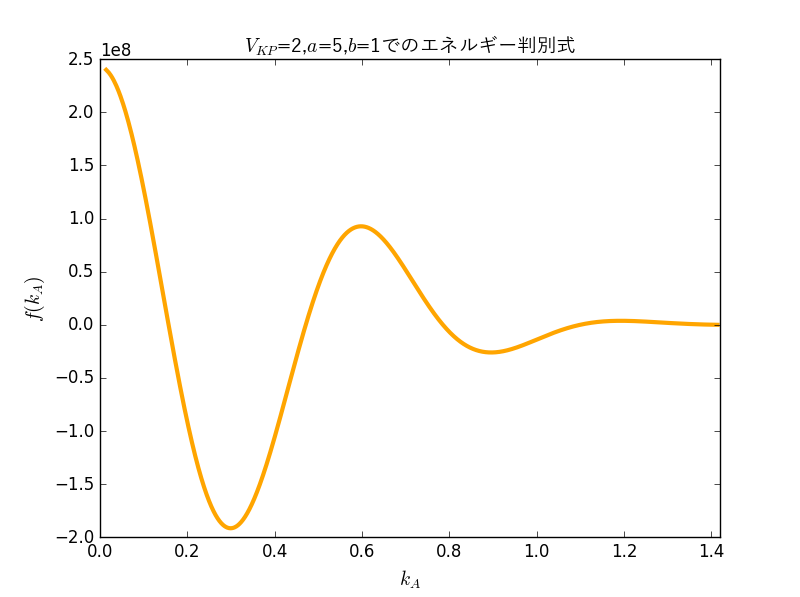
\includegraphics[width=70truemm]{figure_2.png}
             \caption{$k_A$における$V_{KP},a=5,b=1$の判別式}
             \label{BZ1}
             \footnotesize{
              単位は全て原子単位系。エネルギーはHartreeのエネルギーを単位にしている。
             1Hartreeは水素原子に束縛された電子の古典的なエネルギーに等しい。
             このセットアップは3$\mathrm{\AA}$ 程度の格子定数を持つ
             結晶中に1$\mathrm{\AA}$程度のポテンシャルが並んでいる状況を想定している。}
         \end{minipage}&
        \begin{minipage}[t]{0.45\hsize}
            \centering
            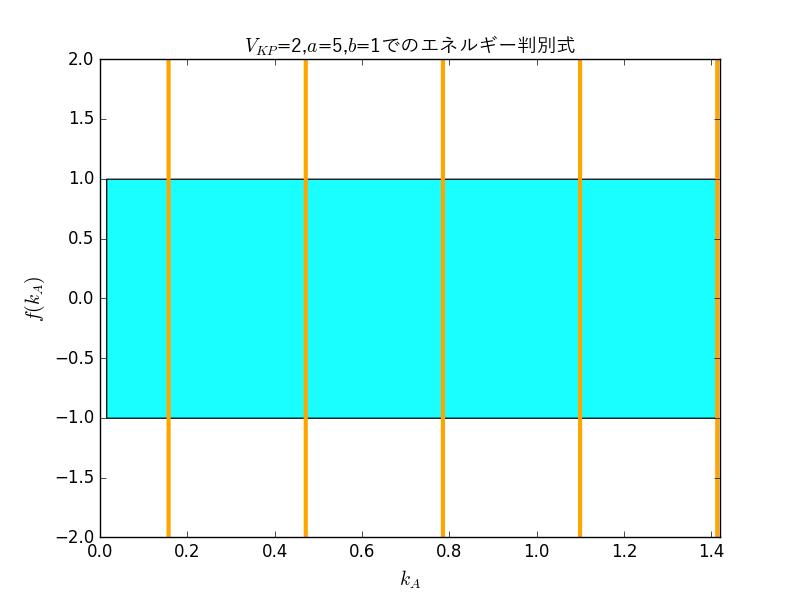
\includegraphics[width=70truemm]{figure_1.png}
            \caption{拡大した判別式}
            \label{BZ2}\footnotesize{\leftline{%
            青い塗りつぶしは$\pm 1$の領域を表す}}
        \end{minipage}
    \end{tabular}
    \end{figure}
    \section{HunagelとZhangの超拡散}
    通常の波束の緩和は標準偏差が\eref{SD}のように時間の一次関数で増大していく。
    しかし、周期ポテンシャルに入れた波束は違った振る舞いをする。\par
    Hunagelは量子が一点から拡散する状況\footnote{波束ではない}を、格子点に局在している量子が隣の格子に放射されるというtight-bindingモデルによって近似した。
    粒子の飛び移り確率は、格子にいる量子を確率の点源(point source)とみなし、
    それから指数関数的に放出されていくというpoint-sourceモデルに基づいて与えられた。\\
    その結果、\eref{MPS}のように分散が拡大していくとした。
    \begin{align}
    P(t) &= \mathrm{e}^{-\Gamma t}\label{source}\\
    M_{PS}(t)&=\int_{0}^{\infty}\:dx\:x^2\int_{0}^{t}\:dt'(-\dot{P}(t'))\delta(x-v(t-t'))\label{variant}\\
    M_{PS}(t)&=v^2\Gamma\int_{0}^{t}\:dt'\mathrm{e}^{-\Gamma t}(t-t')^2\nonumber\\
    M_{PS}(t)&=v^2\left(t^2-\frac{2}{\Gamma}t+\frac{2}{\Gamma^2}-\frac{2}{\Gamma^2}\mathrm{e}^{-\Gamma t} \right)\label{MPS}
    \end{align}
    \eref{MPS}を見ると、$t/\Gamma \ll 1$の状況でかっこ内の第一項以外が消えるため、
    分散が$t$の2乗に比例して増加していくことを説明できる。
    \footnote{\eref{source}の形を$P(t)=1-\Gamma t$にすると、分散が完全に$t$の2乗に比例するようになる。}\par
    Hunagelは$t$の2乗に比例しない因子をHeyperballisticな拡散と呼んだ。
    パラメータ$\Gamma$は時間のスケール因子であり、$\Gamma$を変えることによって様々な時間スケールにモデルを当てはめることができる。
    Zhangはこのモデルをtight-bindingなKronig-Pennyモデルに当てはめ、波束の緩和を計算した。
    その結果、Kronig-Pennyモデルについても\fref{Zhang}のように、
    分散が時間の2乗に乗らない拡散が見られ、ZhangはこれをHeyperdiffusionと呼んだ。
    \begin{figure}[h]
      \centering
      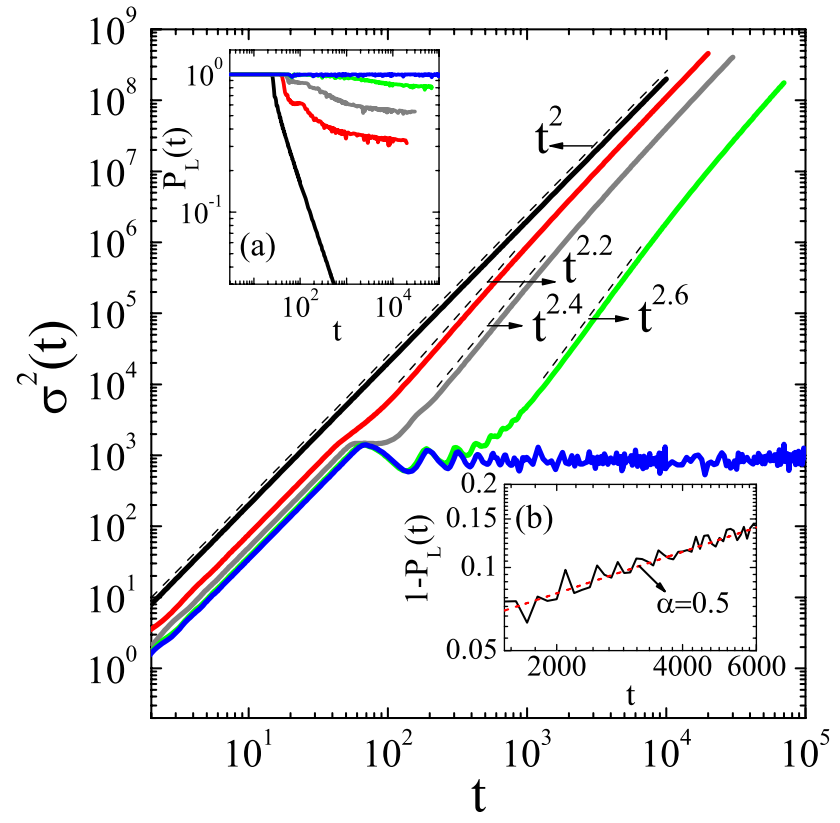
\includegraphics[width=70truemm]{figure_3.png}
      \caption{ZhangによるHeyperdiffusionの計算結果}
      \label{Zhang}
      \footnotesize{横軸は時間、縦軸は分散を表している。
      上から順にポテンシャルが強くなった場合の結果を示している。}
    \end{figure}
    \chapter{結果}
    Kronig-Pennyポテンシャルの簡単な場合として、二枚の壁がある構造を作り、Schrödinger方程式を数値的に計算した。
    その結果、\fref{plt}を得た。
    \begin{figure}[h]
      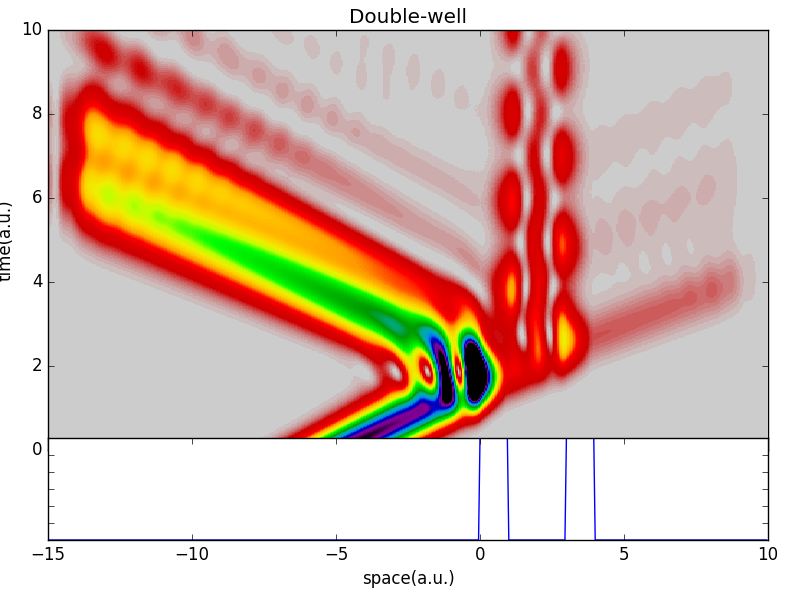
\includegraphics[width=70truemm]{figure_4.png}
      \caption{確率の時空間分布}
      \label{plt}
    \end{figure}
    この結果から、一度壁に侵入した粒子は反射波と透過波に分かれるが、その後も透過反射を繰り返し、
    二次的、三次的な波が井戸から放出され続けていることがわかる。
    そのため、直接反射波と二次、三時反射波の間には時間間隔が存在している。\par
    また、壁の中央からもう一方の壁の中央までの範囲に粒子が存在する確率を計算したところ、\fref{center1}を得た。
    \begin{figure}[h]
      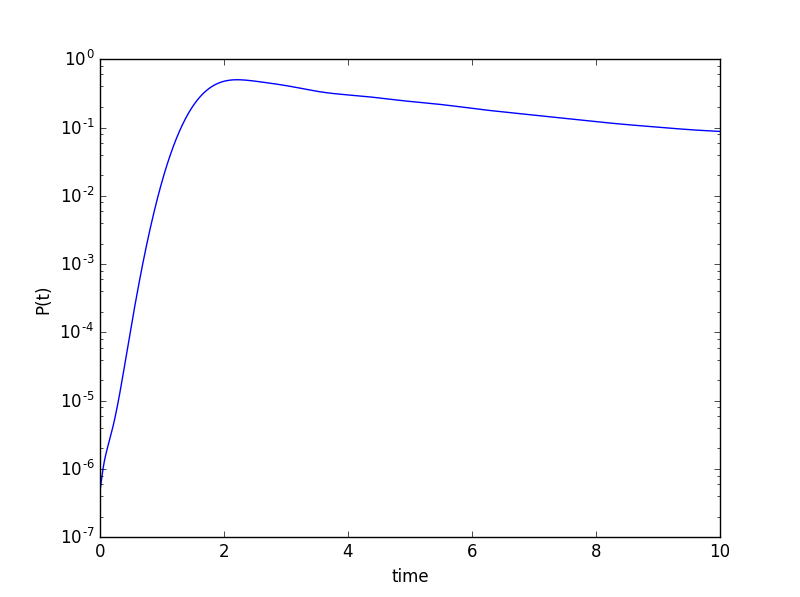
\includegraphics[width=70truemm]{figure_5.png}
      \caption{井戸付近にいる確率の時間推移}
      \label{center1}
    \end{figure}
    波束が侵入した
    この結果から、井戸中央付近に存在している確率は指数関数的に減少していくことがわかる。
    Hunagelによるpoint-source近似の結果がZhangのHeyperdiffusionにも現れた原因として、
    Kronig-Pennyポテンシャルの井戸部分がpoint-sourceと同様の働きを示したことが考えられる。\par
    しかし、長時間の計算を行ったところ異なる傾向が見られるようになった。\par
    それを以下の\fref{center2}に示す。
    \chapter{考察}
    \chapter{schrpyについて}
\end{document}
